\documentclass[10pt,twocolumn]{article}
\usepackage[margin=0.85in]{geometry}
\usepackage{graphicx}
\usepackage{amsmath}
\usepackage{booktabs}
\usepackage[colorlinks=true,allcolors=blue]{hyperref}
\usepackage{caption}
\captionsetup{font=small,labelfont=bf}

\title{\vspace{-1.2em}\textbf{Breakdown voltage and its temperature coefficient\\
for a cryogenically operated SiPM}\\[0.3em]
\large A single-photoelectron charge calibration across three cooldowns}
\author{\normalsize Internal characterisation note}
\date{\normalsize July 2023}

\begin{document}
\maketitle

\begin{abstract}
\noindent
We calibrate the single-photoelectron response of a silicon photomultiplier
operated in a cryostat at three temperatures and extract its breakdown voltage
at each, together with the temperature coefficient
$\mathrm{d}V_{bd}/\mathrm{d}T$. The observable is the charge separation between
the noise and first-photoelectron populations of the integrated-pulse spectrum,
measured in ADC$\cdot$ns, which is independent of the uncalibrated analogue gain
of the readout chain. Breakdown voltage is obtained by extrapolating that
separation against bias to zero, about 6~V below the lowest measured
bias point. We obtain $V_{bd} = 43.037 \pm 0.052$, $43.972 \pm 0.062$ and
$45.073 \pm 0.027$~V at measured temperatures $-98.58$, $-77.67$ and
$-57.72~^\circ$C, and
$\mathrm{d}V_{bd}/\mathrm{d}T = 50.4 \pm 2.2~\mathrm{mV/K}$.
The dominant systematic is not statistical: within each cooldown the bias
ladder was stepped while the cryostat was still drifting, so bias and sensor
temperature are correlated at $\rho > 0.98$ and a fit against bias alone
absorbs part of the temperature dependence into the intercept. Correcting for
that correlation moves $V_{bd}$ by $+0.07$ to $+0.10~\mathrm{V}$, comparable to
the entire spread between defensible analysis methods, and is the single
decision that most affects the result.
\end{abstract}

\section{Motivation}

A SiPM's gain is set by its over-voltage $\Delta V = V_{bias} - V_{bd}$, and
$V_{bd}$ moves with temperature. Any detector that operates SiPMs cold must
therefore know $V_{bd}(T)$ before it can choose a bias set point, equalise gain
across channels, or fix a counting threshold: everything downstream inherits
that calibration. The measurement is routine in the sense that many groups
perform it, and load-bearing in the sense that an error in it propagates
everywhere. Published characterisations of cryogenic SiPMs describe the same
procedure, at liquid-xenon temperature~\cite{ostrovskiy2015} and warm-and-cold
as production QA~\cite{ds20k2026}. This note is a bench measurement on a single
device, carried out at three cryostat setpoints in one campaign of runs.

\section{Data and setup}

The device under test is read out on channel 3 of a CAEN DT5720 desktop
digitizer (250~MS/s, 12-bit, 2~V$_{pp}$ input range) through a
cold preamplifier and a warm second stage. Two further channels carry the
trigger companions and are not used here. The analogue chain was never
calibrated against a known charge, so no conversion to electrons is attempted
and every charge quantity in this note is quoted in ADC$\cdot$ns.

Acquisition covers four cooldowns at controller setpoints $-102$, $-95$, $-78$
and $-58~^\circ$C. At each setpoint a ladder of bias voltages was stepped in
1~V increments, and each bias point was recorded several times at
different leading-edge trigger thresholds. In total 172 files were written,
each holding 700 events of 1024 samples per channel. Cryostat temperatures were
logged independently of the digitizer throughout.

Files are written in the DT5720 standard-firmware event format: four 32-bit
header words carrying the event size, the channel mask, an event counter and a
trigger time tag, followed by the sample payload with two 12-bit samples packed
into each 32-bit word, the earlier sample in the low half. We established this
layout from the manufacturer's documentation and then checked it against the
files rather than accepting it: the record length divides every file exactly,
event counters are contiguous, trigger time tags advance monotonically, and the
event-averaged pulse is smooth. That last check is the one that matters. Per
event, the minimum, maximum and sum of the samples are identical under a
reversal of the packing order, so only the pulse shape distinguishes the two
readings --- and the reversed order produces a visibly serrated waveform whose
mean absolute second difference is three times larger.

\section{Method}

\subsection{Pulse charge}

For each event we fit a low-order polynomial baseline through the sample range
ahead of the pulse and integrate the baseline-subtracted waveform over a fixed
gate. Figure~\ref{fig:waveform} shows the event-averaged pulse; it peaks at
sample 470, i.e.\ 1880~ns into the record, and the gate is
placed around that peak. Block means rather than medians are used for the
baseline: the samples are 12-bit integers with a baseline spread of a couple of
counts, and a median snaps onto integer steps and shifts every area by a
constant.

\begin{figure}[t]
\centering
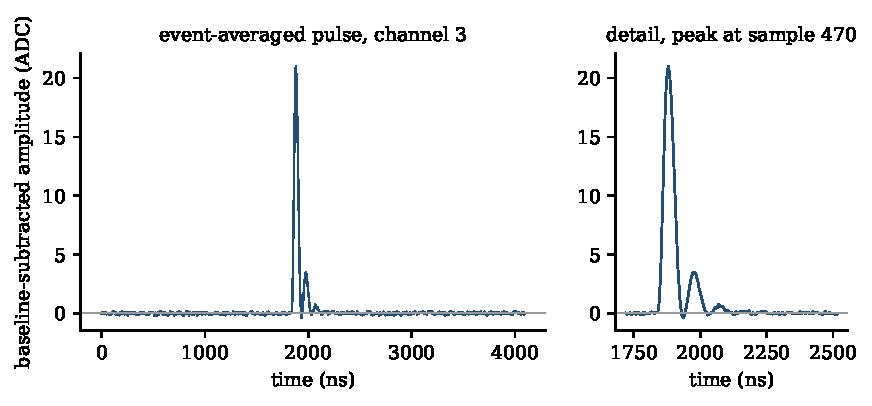
\includegraphics[width=\columnwidth]{figures/fig1_waveform.pdf}
\caption{Event-averaged, baseline-subtracted pulse on the device under test,
with the peak region on the right. The pulse is resolved on the 4~ns
sampling grid and its shape is what distinguishes the correct sample-packing
order from its reversal.}
\label{fig:waveform}
\end{figure}

\subsection{The observable}

The spectrum of integrated charges is not a single peak. It carries a noise
population from events in which the device under test did not fire, a
first-photoelectron population, and higher orders that at these statistics hold
too few events to locate a centre. We therefore measure the \emph{separation}
between the noise and first-photoelectron populations, not the absolute
position of either.

This choice is not cosmetic. The noise population does not sit at zero: it
carries whatever residual offset the baseline estimator leaves behind, and that
offset is common to both populations, so it cancels in the difference and does
not cancel in an absolute peak position. Reporting a peak position instead of a
separation carries that offset into an extrapolation several volts long. During
this analysis the two definitions were seen to disagree by of order
0.1~V in $V_{bd}$ purely by measuring different quantities.

\subsection{Acquisition thresholds}

Each bias point was recorded at several trigger thresholds, and the threshold
selects which events reach the file. That is a selection on pulse amplitude,
and if it were also selecting on integrated charge it would bias the
separation. Figure~\ref{fig:threshold} shows the extracted separation against
threshold at every bias point of all three calibrated cooldowns. It is flat
within the fit errors at every setting; we therefore merge thresholds per bias
point and carry the spread across them as a systematic rather than assuming
it away.

\begin{figure*}[t]
\centering
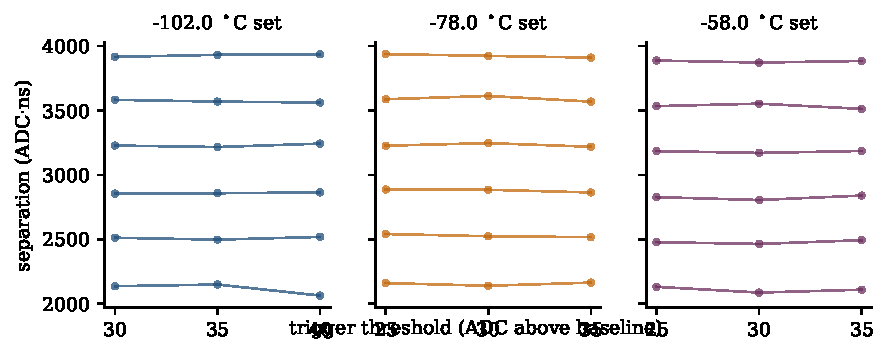
\includegraphics[width=\textwidth]{figures/fig2_threshold.pdf}
\caption{Extracted noise-to-1PE separation against acquisition threshold, one
trace per bias point, for the three calibrated cooldowns. Flat within errors:
the threshold selects events by amplitude but does not measurably select on the
charge observable.}
\label{fig:threshold}
\end{figure*}

\subsection{Which cooldowns can be calibrated}

Breakdown voltage is the intercept of separation against bias, so a cooldown
needs a ladder of distinct bias voltages before it can carry one. Three of the
four cooldowns do: $-102~^\circ$C spans 49--54~V,
$-78~^\circ$C spans 50--55~V, and $-58~^\circ$C spans
51--56~V, each in 1~V steps at three thresholds. The
$-95~^\circ$C cooldown sits at a single bias voltage. No number of events fixes
a slope from one abscissa, so it cannot carry an independent breakdown voltage
and we do not report one for it.

\subsection{Temperature}

The temperature used for each cooldown is the mean of the cryostat log over
that cooldown's acquisition window, with the standard deviation over the same
window quoted alongside it. The controller setpoint is not used as a
measurement: the setpoints and the logged means differ by up to
3.4~K, which is large enough to move the coefficient well outside
its uncertainty.

\section{The temperature--bias confound}

\begin{table}[t]
\centering
\small
\begin{tabular}{lrrr}
\toprule
 & $-102~^\circ$C & $-78~^\circ$C & $-58~^\circ$C \\
\midrule
$\rho(V, T)$ within campaign & 0.997 & 0.988 & 0.989 \\
$\mathrm{d}T/\mathrm{d}V$ (K/V) & 0.26 & 0.24 & 0.21 \\
$\Delta V_{bd}$ if uncorrected (V) & $-0.071$ & $-0.103$ & $-0.101$ \\
\bottomrule
\end{tabular}
\caption{Within each cooldown the bias ladder was stepped while the cryostat
was still settling, so bias and sensor temperature are almost perfectly
correlated. A fit against bias alone therefore absorbs part of the temperature
dependence and biases the intercept low.}
\label{tab:confound}
\end{table}

The bias ladders were stepped upward while the cryostat had not fully settled.
Within each cooldown, bias voltage and logged temperature are consequently
correlated at $\rho > 0.98$ (Table~\ref{tab:confound}), with the sensor moving
0.21--0.26~K per volt of bias.

This matters because the separation depends on both quantities. Fitting it
against bias alone lets the fit absorb part of $\mathrm{d}Q/\mathrm{d}T$ into
the slope, which tilts the ladder and moves the intercept. Switching the
correction off in our own pipeline moves $V_{bd}$ by $-0.071$, $-0.103$ and
$-0.101$~V at the three cooldowns --- always low, and largest where
the ladder is longest.

We therefore fit against a drift-corrected bias,
\begin{equation}
X_i = V_i - \beta\,(T_i - T_c),
\end{equation}
where $T_i$ is the logged temperature at bias point $i$, $T_c$ the campaign
temperature, and $\beta$ the breakdown-voltage temperature coefficient itself.
Because $\beta$ is what we are measuring, it is iterated to self-consistency
across the three cooldowns rather than assumed. Four iterations suffice.

The size of this correction deserves emphasis: at
0.07--0.10~V it is comparable to the entire spread between
defensible analysis pipelines applied to the same files. An analysis that
ignores it is not wrong by a rounding error; it is wrong by about as much as
the method choice itself can justify.

\section{Results}

\begin{figure}[t]
\centering
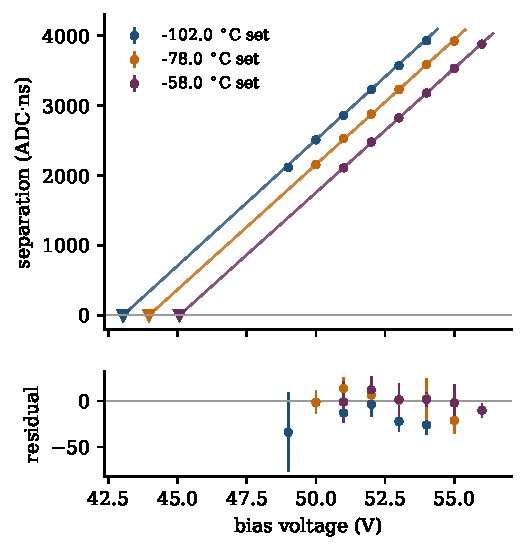
\includegraphics[width=0.92\columnwidth]{figures/fig3_gain_vs_bias.pdf}
\caption{Noise-to-1PE separation against bias voltage for the three calibrated
cooldowns, with the fitted line extrapolated to its intercept (triangles) and
residuals below. The intercept sits about 6~V below the lowest
measured point, so the slope carries a long lever arm onto $V_{bd}$.}
\label{fig:gain}
\end{figure}

Figure~\ref{fig:gain} shows the separation against bias at each cooldown with
the fit and its residuals. The relation is linear across the measured range;
reduced $\chi^2$ values are 0.53, 0.64 and 0.10, and the residuals scatter
rather than following a shape. We fit a straight line for that reason and note
what the alternative would cost: the intercept lies about 6~V below
the lowest measured bias point, so a one per cent error in the slope moves
$V_{bd}$ by roughly 0.085~V, and a quadratic through the same points
would move it by 0.3--0.6~V. Curvature has to be established
before it is followed, not inferred from residuals inside the measured range.

\begin{table}[t]
\centering
\small
\begin{tabular}{lrrr}
\toprule
Setpoint ($^\circ$C) & $-102$ & $-78$ & $-58$ \\
\midrule
Measured $T$ ($^\circ$C) & $-98.58$ & $-77.67$ & $-57.72$ \\
$\sigma_T$ over window (K) & 0.86 & 0.48 & 0.40 \\
Slope (ADC$\cdot$ns/V) & 360.6 & 357.7 & 356.1 \\
$V_{bd}$ (V) & 43.037 & 43.972 & 45.073 \\
$\sigma_{V_{bd}}$ (V) & 0.052 & 0.062 & 0.027 \\
$\chi^2/\mathrm{dof}$ & 0.53 & 0.64 & 0.10 \\
\bottomrule
\end{tabular}
\caption{Per-cooldown calibration. Temperatures are means over each cooldown's
acquisition window from the cryostat log, not controller setpoints.}
\label{tab:results}
\end{table}

Table~\ref{tab:results} collects the per-cooldown results.
Figure~\ref{fig:vbdt} shows $V_{bd}$ against measured temperature. A weighted
straight-line fit gives
\begin{equation}
\frac{\mathrm{d}V_{bd}}{\mathrm{d}T} = 50.4 \pm 2.2~\mathrm{mV/K},
\end{equation}
with residuals consistent with the per-cooldown uncertainties. The measured
slope of the separation against bias is stable across cooldowns to better than
1.3\,\%, as expected if the device's over-voltage response is
temperature-independent to first order over this range.

\begin{figure}[t]
\centering
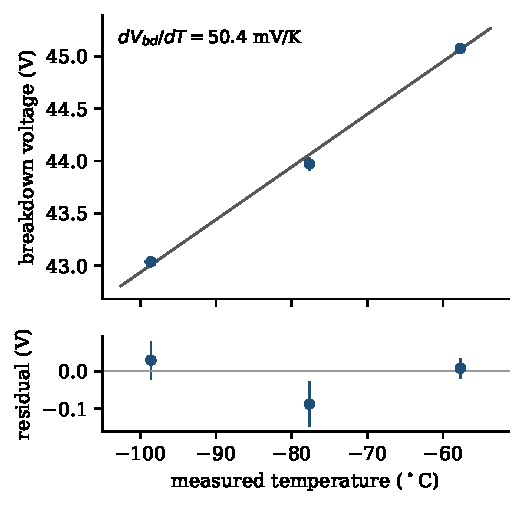
\includegraphics[width=0.92\columnwidth]{figures/fig4_vbd_vs_temperature.pdf}
\caption{Breakdown voltage against measured cryostat temperature, with the
weighted fit and residuals. Horizontal bars are the temperature spread over
each acquisition window.}
\label{fig:vbdt}
\end{figure}

\section{Uncertainties}

Per-setting uncertainties come from the fit covariance of the population
centres and from the spread across the acquisition thresholds at that bias
point, whichever is larger. These propagate into the per-cooldown extrapolation
and from there into the coefficient.

The systematics that matter here are correlated across cooldowns: a change of
analysis choice moves all three breakdown voltages in the same direction. We
therefore propagate them by recomputing the temperature slope under each
variation rather than by inflating the per-cooldown errors and refitting, which
would treat them as independent and overstate the result. Varying the
integration gate across its plateau, the baseline model, and the estimator used
to locate the two populations moves the coefficient by less than
1.5~mV/K in total. The drift correction of
Section~4 is the exception and is not a variation but a correction: leaving it
out is an error, not an alternative.

One limitation is worth stating plainly. The reference against which any such
analysis can be checked is the spread of defensible methods applied to these
same files, not an independently known truth. Two competent analyses of this
dataset differ by up to 0.14~V in $V_{bd}$, and that number, rather
than the fit uncertainty, is the honest scale on which a result should be
judged.

\section{Conclusion}

The device's breakdown voltage rises from 43.04~V at
$-98.6~^\circ$C to 45.07~V at $-57.7~^\circ$C, giving
$\mathrm{d}V_{bd}/\mathrm{d}T = 50.4 \pm 2.2~\mathrm{mV/K}$ over
that range. The calibration rests on three decisions more than on any fitting
detail: measuring a population \emph{separation} rather than a peak position,
taking temperatures from the cryostat log rather than the controller setpoint,
and correcting the correlation between bias and temperature within each
cooldown before extrapolating. The first two are matters of definition; the
third is worth 0.07--0.10~V and is easy to miss, because a fit
that ignores it looks entirely healthy.

\begin{thebibliography}{9}
\small
\bibitem{ostrovskiy2015}
I.~Ostrovskiy \textit{et al.},
``Characterization of Silicon Photomultipliers for nEXO,''
\textit{IEEE Trans.\ Nucl.\ Sci.} \textbf{62} (2015) 1825,
\href{https://arxiv.org/abs/1502.07837}{arXiv:1502.07837}.

\bibitem{ds20k2026}
DarkSide-20k Collaboration,
``Construction and characterisation of the DarkSide-20k veto silicon
photo-multiplier tiles,''
\textit{Eur.\ Phys.\ J.\ C} (2026),
\href{https://arxiv.org/abs/2604.02551}{arXiv:2604.02551}.

\bibitem{caen}
CAEN S.p.A., \textit{DT5720 Desktop Waveform Digitizer --- Technical
Information Manual}, rev.~5.

\end{thebibliography}

\end{document}
